\chapter{TSP-Cube 算法}

针对 MR-Cube 的不足,本文提出了 TSP-Cube 数据立方计算方法。TSP-Cube 借鉴了 \cite{tao2013minimal} 中将 TeraSort 与 GroupBy的结合,将TeraSort 的思想用于数据立方计算中数据的划分。同时,提出使用PipeSort 替换BUC算法,充分利用MapReduce框架的特性,计算同一个reduce函数内多个group的聚集。并且针对层次型数据集的特征,提出更为简单有效的 pipeline 生成方案。


\section{TeraSort与GroupBy}

由于TSP-Cube借鉴了 \cite{tao2013minimal} 中 TeraSort 与 GroupBy的结合,因此这里对使用TeraSort计算GroupBy做一个简单的介绍。它们两者的结合是为了解决计算倾斜数据集的GroupBy时,由于各个 reducer 上数据的不均匀,导致部分 reducer 运行时间过长的问题。

在阐述TeraSort与GroupBy结合前,首先阐述使用 MapReduce 计算 GroupBy 的一般方法(称为Base GroupBy)。这个方法与 使用 MapReduce 计算数据立方的 Naive 方法类似。在 数据立方中,mapper的输出是每一条记录与所有 region 的映射。而在 GroupBy 中,仅需要与一个 region,即 GroupBy 的 region 映射即可。例如记录 e1=[a0, b0, c0, d0, m0],其中a0, b0, c0, d0对应的属性是维属性,m0 对应的属性是度量属性。当前操作是 GroupBy(B),那么对于这条记录输出的 key 为 b0,value 为 m0。具有相同的 key 值的数据会被分发到同一个 reducer 上计算,也就是具有相同 group\_value 的数据会被分发到同一个 reducer 上计算。如果数据集是倾斜的,也就是这个 region 内有一些特别大的 group,将导致一些 reducer 分发到大量的数据,而一些 reducer 分发到较少量的数据,负载不均衡导致最终计算效率的下降。

将 TeraSort 与 GroupBy结合,目的是对 region 内较大的 group 进行划分,从而将一个 group 分发到多个 reducer 上进行计算,降低负载不均衡。TeraSort 的采样以及分界点的选择恰好能对大的 group 进行划分。论文中以度量函数 SUM 作为例子,采样的数据是维属性与记录编号组成的组合键。也就是采样的key是[group\_value, tuple\_id]这样的组合键。之后的操作与 TeraSort 类似,将采样的数据发到一个 reducer 上,采样的数据会被排序,然后根据 reducer 的数量选取分界点。由于这里的key是复合键,因此在 group\_value 相同的情况下会比较 tuple\_id。也正因为这个tuple\_id,较大的 group 才能被划分。

图 \ref{ts_groupby} 是使用 TeraSort 方法对采样的数据进行划分的示例。图中每个矩阵表示一个 group,矩阵越大,表示采样数据中具有相同 group\_value 的样本越多。红色的线表示分界点。分界点之间的间距是基本相同的,对于较大的 group 很有可能有一个或多个分界点落在其上,正好将 group 进行了划分。若采样的key中只有 group\_value,而没有 tuple\_id,那么对于一个大 group,就算有多个分界点落在其上,但分界点的值都是相同的,这样的分界点就没有意义了。

图中每个分块都标有数字,各个分界点之间有多个分块,两个分界点之间的区域称之为划分区域。在同一个划分区域内的不同分块都会分派到同一个 reducer 上进行计算。但由于 group\_value 的不同,即使这些分块分到同一个 reducer 上,也会调用多次 reduce 函数。只有同一个 reducer 中具有相同 group\_value 的数据才会放在同一个 reduce 函数中进行计算。

\begin{figure}[!ht] 
\centering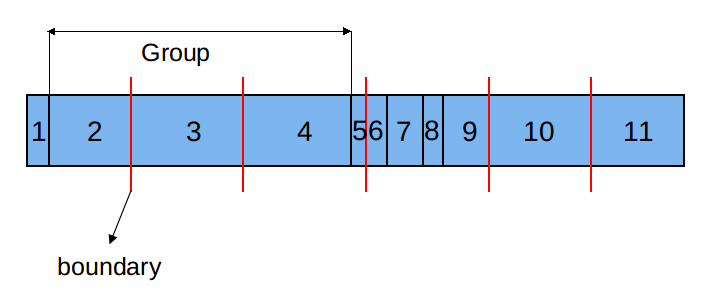
\includegraphics[width=4in]{picture/ch_terasort_mr/ts_groupby} 
\caption{使用TeraSort划分GroupBy的计算}\label{ts_groupby} 
\end{figure}

以上的采样以及选取分界点是第一轮的 MapReduce。第二轮的 MapReduce 与上面提到的计算 GroupBy 的 Base 方法类似,只是 key 的输出不仅仅是 group\_value,还需要tuple\_id。这样才能通过与分界点的比较确定数据要分发到某个确定的 reducer 上。使用 TeraSort 计算 GroupBy 还需要第三轮的 MapReduce,因为在上一轮的计算中,大的 group 被划分了,因此第三轮的 MapReduce 是对被划分的 group 进行合并。

以上 是 \cite{tao2013minimal} 中提到的将 TeraSort 与 GroupBy 结合的方法,但论文中忽略了一个非常重要的关键点,那就是 MapReduce 的 combiner。Combiner的作用在前面的章节中有提及,它是 MapReduce 一个重要的机制,它等同于本地的 reducer。它会对 mapper 的输出进行一次本地的 reduce 计算,然后再将数据发到相应的 reducer 上,这样可以减少网络传输的数据量和reducer 的计算量。对于代数度量函数,combiner 可以在本地对同一个 group 内的数据进行一次计算,将一个 mapper 上同一个 group 内的数据压缩成一条记录发送到 reducer 上,而不是将这个 group 内的数据直接发送到 reducer上,由于mapper的数量是有限的,因此reducer获得的同一个group内的数据也是有限的。那么就不存在reducer之间严重的负载不均衡问题了。

倘若不使用 combiner,TeraSort 和 GroupBy 的结合是非常有用的。但是若使用了 combiner,即使是使用 Base 的方法计算 GroupBy,对于代数度量函数,也基本不存在 reducer 上数据不均匀的情况。 这种情况下,TeraSort 就没有使用的必要了。但这并不是完全否定 TeraSort 对 GroupBy 的作用,因为对于整体性度量函数,combiner无法发挥作用,那么TeraSort 对数据的划分就有非常大的作用了。在实验章节中,将会分别比较整体性度量与代数度量在不同算法下的效率与各个reducer上数据的分布,从而分析出 TeraSort 适用的场景。


\section{TSP-Cube}

借鉴 TeraSort与GroupBy结合的方法,并且针对MR-Cube的一些不足,本文提出了TSP-Cube 算法。TSP-Cube 将 TeraSort、PipeSort 与分布式数据立方结合,从数据划分和合并计算这两个方面一同提高数据立方的计算效率。

TSP-Cube 借鉴了 MR-Cube 的一些思路,例如整体性度量的划分、Batch Area,同时对它存在的不足进行了改进。TSP-Cube使用 TeraSort 的思想,利用分界点确定要划分的group,从而改进了 MR-Cube 中由于一个region内有大group,而对region内所有group都进行划分的方法,避免了对小 group 的不必要的划分。TSP-Cube 使用分界点对大group进行划分,与MR-Cube中使用取模的方式相比,数据划分更均匀。同时,TSP-Cube 使用PipeSort 替换了了MR-Cube 中的BUC,充分利用了 MapReduce 框架的特性,并且针对层次型的数据集,提出了一个更简单有效地形成 Pipeline 的方法。

\subsection{TeraSort与分布式数据立方}

%TSP-Cube针对MR-Cube的改进主要包括两个方面,一方面是使用TeraSort的思想对数据进行划分,另一个使用Pipesort计算多个group的聚集。这一节阐述将TeraSort运用于数据立方计算中,对数据进行划分。而pipeosrt的使用将在下一节中阐述。

由于 GroupBy 是数据立方的一个子操作,受到 TeraSort 与 GroupBy 结合的启发,TSP-Cube 将TeraSort 与数据立方相结合,并且发现这样的结合能解决上一章中提到的 MR-Cube 存在的一些问题。


%\subsection{数据采样与划分}

对于整体性度量函数,无论是 MR-Cube 还是 TSP-Cube 都要解决一个问题,那就是各个reducer之间负载均衡的问题,而解决这个问题的方法都是对大 group 进行划分。在 MR-Cube 中是通过采样,然后根据采样数据中 group 的大小确定 region 是否为 reducer-unfriendly region。对于 reducer-unfriendly 的region,region 内的 group 都需要进行划分,无论group大小与否。这样会对小group产生不必要的划分,其最根本的原因是划分点的数量。在MR-Cube中,同一个region内所有的group都拥有相同的划分因子,即划分点数量,这些划分点保证大group能够被划分,但对于小group而言,则使用了过多的划分点。而在TSP-Cube中,即使只使用与reducer数量相同的划分点,也能划分大group,并且令各个reducer负载均衡。

对于 TSP-Cube,运用 TeraSort 的思想,同样需要采样,然后对采样数据排序,选取分界点。这些分界点的选取,限定了落入各个redcuer中的数据的数据范围,更重要的是分界点落在大group上,能对大group进行划分,将一个大group拆分到多个reducer上,从而使各个reducer之间的数据均匀,避免一两个reducer负载过重。

采样的key值非常重要,因为它关系到分界点的选取、group的划分以及第二轮 MapReduce 计算时 reducer 之间数据的均匀性。在 GroupBy 的场景下,采样的 key 是 [group\_value, tuple\_id] 这样的复合键,在数据立方的计算中,由于计算的不仅仅是一个 region,因此采样的 key 更为复杂。并且\cite{tao2013minimal} 中讨论的度量函数仅是 SUM,而这里还需要考虑到整体性度量函数。

首先考虑region的因素。TSP-Cube的采样是为了了解原数据中各个region中各个group的大小,因此样本的key值的出现频率必须要反应group的大小,所以key值必须包含region和group的信息。因此选择region\_id 和group\_value 组成复合键作为key值。将各个 region 转化成字符串并且排序,然后对它们编号,即可得到 region\_id。这样使用[region\_id, group\_value] 复合键即可表示一个指定 region 内指定的 group。但仅用这两个值对于大的group是无法划分的。因为若两个分界点落在同一个region的同一个group内,这两个分界点的值是相同的,因此这里需要加入更多的信息。这个信息与度量函数有关。

对于代数度量,由于数据划分不受限制,因此数据不需要按照某个特定的属性进行划分。所以这里参考\cite{tao2013minimal},选择 tuple\_id 作为 key 值的一部分。tuple\_id 一般是数据的主键,主键是无重复的。这种情况下,一个 group 内若有多个分界点,分界点的值也是不同的。因此,对于代数度量函数,采样时的key值为 [region\_id, group\_value, tuple\_id]。但其实对于代数度量,使用 TeraSort 计算数据立方会碰到与 GroupBy 类似的问题,由于 MapReduce combiner 的作用,对于mapper的输出可在本地进行一次reduce计算,令同一个group内的数据被压缩成一条记录输出,因此reducer接收到的数据量是有限的。所以即使是计算较大的数据集,也不会出现 reducer 之间数据不均匀的情况。这一点在之后的实验中也充分地说明了。因此 TSP-Cube 着重解决整体性度量函数的问题。

对于整体性度量,随意的数据划分对它的计算很可能是无任何帮助的。在这里,可使用 \cite{nandi2011distributed} 提出的部分代数度量(Partially Algebraic Measure)。也就是根据不同的整体性度量函数按照某个或多个特定的属性值进行划分,而这个属性值在多数情况下都是度量属性值。因此,对于整体性度量函数,采样时的key应为 [region\_id, group\_value, measure\_value]。这种情况下,即使一个 group 内有多个分界点,因为度量值的不同,分界点的值也不同。这样就能划分一个大group。例如计算 COUNT(DISTINCT(uid)),uid 为度量值,那么采样的key值	为 [region\_id, group\_value, uid]。若一个group是一个较大的group,它很可能被分界点划分成多个分块。由于分界点的值中有uid,因此同一个group内相同的 uid 必定会划分到同一个分块中,两个不同的分块中必定无相同的 uid。对于每个分块可以计算各自的 COUNT(DISTINCT(uid)),这个中间结果是一个整数,最后对每个分块的结果做累加即可。

图\ref{tscube_picture} 为 TSP-Cube 的采样与分界点的选取。每一个矩阵表示一个 group,相同颜色的矩阵表示同一个 region 内的 group。红色的直线表示分界点。从图中可看出分界点更容易落在较大的矩形上,并且group 越大,分界点就可能越多。因此大的 group 更容易被划分,从而分派到多个 reducer 上进行计算。这里与 GroupBy 的情况也是类似的,虽然一个 reducer 中有多个分块,但是只有相同region\_id 和 group\_value 的数据才会在同一个 reduce 函数上进行计算。

\begin{figure}[!htb] 
\centering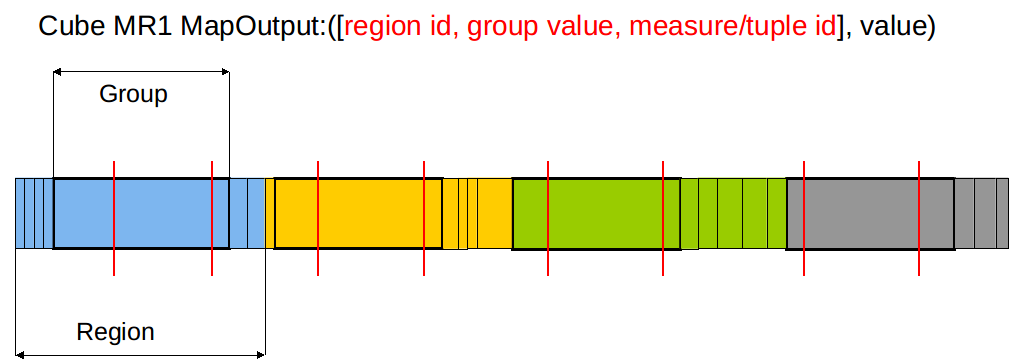
\includegraphics[width=6in]{picture/ch_terasort_mr/tscube_picture} 
\caption{TSP-Cube的采样与分界点的选取}\label{tscube_picture} 
\end{figure}

根据以上的方法所选取的分界点规定了每个 reducer 所要处理的数据范围,更重要的是对大group进行了划分。group 越大,采样中所占的比例也越大,那么分界点越容易落在其上。因此能达到大group被划分的目的。而对于分界点数量,若有 t 个reducer,则至少要选取 t-1 个分界点。但其实可以选择更多分界点,只要保持是t的倍数减1的关系即可。这个倍数该如何选择,可根据 reducer limit 进行估算。reducer limit 是 \cite{nandi2011distributed} 中提出的概念,它指的是一个reducer最多可处理的记录数量,是一个估算值。它通过reducer的内存大小以及一条记录的大小,从而估算reducer的负载量。

假设数据集中记录总数为 TotalSize,$\frac{TotalSize}{ReducerLimit}$ 是估算若每个reduce函数处理的数据量都不超过其负载量,则整个数据集需要调用多少次reduce函数。这里将这个reduce函数的数量作为TeraSort中分界点的数量。因为采样中的分界点是为了划分实际计算中的group。若分界点选取过少,即使数据划分均匀,但可能出现一个reduce函数依然要处理一个大group的情况;若分界点选取过多,则可能会出现MR-Cube中不必要划分的问题。因此这里从整体的角度出发,确定分界点的数量。用上述的方式确定分界点数量,既能令每个分块都不超过reduce函数的负载量,又可以避免对小group的划分。

由于分界点的数量必须是t的倍数减1(t为reducer的数量),因此这里对上述的估算稍微做一些放大,保证倍数关系。因此最终选取的分界点数目为$\lceil \frac{\frac{TotalSize}{ReducerLimit}}{t} \rceil \times t -1 $。

%但这个倍数到底如何选择是最佳的,目前仍未从理论上给出可行的证明,因此目前可作为一个参数供用户自行选择。

%可参考 MR-Cube 的划分因子 \cite{nandi2011distributed} 使用以下的方法进行估算。

%假设数据集中记录总数为 TotalSize,样本的记录总数为 SampleSize,样本中最大的group所包含的记录数为 S,由这三个值估算出,数据集中最大的group所包含的记录数为 $T = \frac{S\times TotalSize}{SampleSize}$。若有 t 个reducer,当选取 t-1 个分界点时,落在最大的 group 上的分界点的数量为 B。对最大的 group 划分,可根据 reducer limit 估算划分因子,$PartitionFactor = \frac{T}{ReducerLimit}$。那么最终要划分的数量为 $\left( \frac {PartitionFactor}{B} - 1 \right) \times ReducerNumber$。

%对以上方法最直观的理解是,若使用最少的分界点划分时,最大的group的每个子块却依然超过了reducer limit,则需要对每个子块再进行划分。而再划分的数量通过 reducer limit 与大group 内的记录数估算获得,即$PartitionFactor$。而 $\frac {PartitionFactor}{B} - 1 $ 是计算大group内每个已划分的子块中还需要添加多少分界点。最后将该值乘以总的 reducer 的数量,即是最后样本所需要的总的分界点数目。

使用 TeraSort 的采样与数据划分方式正好可以解决 MR-Cube 中 group 的划分问题。在 MR-Cube 中,只要一个 region 内有一个大 group,那么这个 region 内所有的 group 都要被划分,无论其他的group大小与否。MR-Cube是使用比实际需要多更多的划分点来保证大group一定能被划分,但牺牲了小group,令小group产生不必要的划分,若大group和小group之间大小差距较大,那么就会产生较多的冗余划分,也加重了之后的合并操作。而TSP-Cube则正好相反,它减少划分点的使用,最少的情况下,只使用与reducer数量相同的划分点,但却能令划分点较为精准地落在需要划分的group上,从而减少不必要的划分,同时也保证了各个reducer之间的数据均匀性。

TSP-Cube之所以能令划分点较为精准地落在需要划分的group上,是因为需要划分的group都是大group,group越大,样本中出现的频率就越高,而分界点是均匀选取的,那么分界点就有很大的概率落在大group上,从而划分大的group。若样本中有较多的大group,分界点一般会落在这些较大的 group 上。对于不落在大 group 上的分界点,则可能落在两个小的 group 之间或者落在小group上。但因为 group 越小,采样中该 group中的数据 出现的频率也越少,那么分界点落在这些小 group 上的概率也就相对较小了。按照上述分析,大部分的分界点都会落在大group上,只有少数的分界点会落在小group上或小group之间。TSP-Cube虽然使用较少的分界点,但依然保证了大group的划分和各个reducer上数据的均匀性,并且避免了 MR-Cube 中出现的不必要的划分。

TSP-Cube使用TeraSort思想解决不必要的数据划分的同时,也解决了MR-Cube中使用取模方法对数据划分可能带来的不均匀性问题。取模是简单有效的哈希函数,但在一些极端情况下,原数据有倾斜性,导致划分后的数据可能依然有倾斜性。例如使用 MR-Cube 的方法计算的划分因子的结果是2,也就是令度量属性值对2取模从而达到数据划分的效果,若需要划分的属性值大部分都是奇数,这样将导致数据划分的失效,数据划分后依然是不均匀的。而使用 TSP-Cube 的方法则可以避免这种情况。因为 TSP-Cube 对数据的划分是基于样本出现的顺序和频率的,即使所有的度量属性值都是奇数,TSP-Cube 依然可以较为均匀地划分数据。


%\subsection{数据立方的计算}

%以上的采样与分界点的选取是第一轮的 MapReduce,也即是对数据的划分。第二轮进行的 MapReduce 是对数据立方的计算。这里先不考虑将多个 group 的数据放在同一个 reduce 函数里计算的情况(即MR-Cube 中提出的 Batch Area),仍采用 Naive 的方法,映射所有的region。TSP-Cube 与 Batch Area 的结合将在下一节中阐述。

%根据使用 TeraSort 对数据进行全局排序以及计算 GroupBy 可看出来,第二轮的 MapReduce 中 mapper 输出的 key 一般与采样的 mapper 所输出的 key 是一致的。因为第一轮 mapper 输出的key中的若干个会被选为分界点,第二轮mapper的输出必须与第一轮保持一致,才可以与分界点进行比较,从而决定键值对落到哪个 reducer 上。而这个与分界点的比较需要重载 MapReduce 中的 Patitioner,将 mapper 的输出与上一轮选取的分界点进行比较,可使用二分查找的方法,确定 mapper 的输出应该落在哪两个分界点之间,从而确定该键值对应该分派到的reducer 的ID。

%在 reduce 阶段,同一个 reducer 内的数据,若具有相同 region\_id 和 group\_value 则会在同一个 reduce 函数内进行计算。此处 reducer 的计算与 Naive 是一样的,因此不再详细说明。


%这里需要为 MapReduce 的机制进行一些说明。在默认的 MapReduce 中,只有具有相同 key 值的数据才会放在同一个 reduce 函数中计算。而在 TSP-Cube 第二轮 MapReduce 中 mapper 输出的 key 值为 [region\_id, group\_value, tuple\_id or measure\_id],是一个复合键。按照默认规定,必须这3个值都相同才能放在同一个 reduce 函数内计算。但其实 MapReduce 的框架为此提供了灵活的变化。用户可重载 GroupPartitioner 函数,此函数是定义在同一个 reducer 内,具有什么特征的数据会被放在同一个 reduce 函数中计算。由于TSP-Cube 的特殊性,这里需要重载 GroupPartioner,规定在同一个reducer内,只要 region\_id 和 group\_value 相同的数据即可放在同一个 reduce 函数内计算。

%最后进行第三轮的 MapReduce,将被划分的数据进行合并。这里合并的方法非常简单,并且实验证明也是很高效的。合并的方法与 MapReduce 做单词统计是类似的,因为第二轮 MapReduce 输出的 key 是 region\_id 和 group\_value,输出的 value 是 measure\_value。因此在第三轮的 MapReduce 中,只要将第二轮输出的数据读入,对相同 region\_id 和 group\_value 的数据做一次合并即可,这个过程与单词统计是一样的。虽然上一轮将部分的 group 进行划分,但是这个划分的数量是有限,因此合并过程中,具有相同 region\_id 和 group\_value 的数据也并不多。


\subsection{PipeSort 与分布式数据立方}

上一节中主要阐述了数据的划分,在这一节中将详细阐述如何使用 PipeSort 将多个 group 放在同一个 reduce 函数里计算,也就是减少数据立方计算过程中,中间数据的产生。 

MR-Cube 提出了 Batch Area 的概念和一些划分 Batch Area 建议遵循的规则,但是并没有给出简单且具体的划分方法。同时 MR-Cube 中使用的是 BUC 对Batch 内的 group 进行计算,但其实这种方法并没有充分利用 MapReduce 框架的特性。因此 TSP-Cube 针对这两点进行改进,TSP-Cube 提出使用 PipeSort 替代 BUC 进行多个group之间的计算,从而与MapReduce有更好的结合;并且特别针对层次型的数据集,提出了简单且有效的划分方法,该方法与 PipeSort 有非常好的整合。

PipeSort\cite{agarwal1996computation} 是 1996 年由 Agarwal 等人提出的一种计算数据立方的方法。Pipe 指的是 Pipeline,即流水线。它是一种自顶向下的计算数据立方的方法。它利用数据的有序性以及多个 group 之间具有共同前缀的特性,对数据只扫描一遍并且使用极少的内存即可计算多个 group 的聚合。

如图\ref{pipesort} 所示,这是一个4维的数据立方其中一种可行的 pipeline 方案。每个虚线框内表示的是一个pipeline。这些 pipeline 之间是共享共同前缀的,例如 $ABCD\rightarrow ABC\rightarrow AB\rightarrow A$ 这样一个pipeline,将数据按照 ABCD 这样的属性顺序排序,再对数据进行扫描,在扫描的过程中可同时计算 ABC、AB、A 的聚合。因为数据已经按照 ABCD 这样的维属性进行排序,那么具有相同 ABC、AB 或者 A 值的数据在顺序上必定会相连的,因此可通过一遍扫描且只使用少量内存即可计算出这 4 个 group 的聚合。

\begin{figure}[!htb]
\centering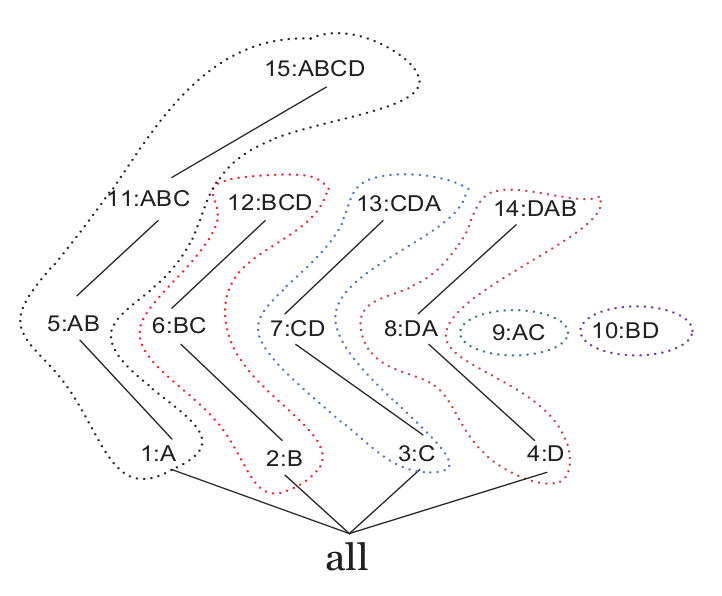
\includegraphics[width=3in]{picture/ch_terasort_mr/pipesort} 
\caption{4维数据立方的划分}\label{pipesort} 
\end{figure} 

正是因为 PipeSort 的有序性以及一次性扫描的特点,它更适合应用于 MapReduce 的框架。因为 MapReduce 默认对数据进行排序,无论用户是否需要,它都会对数据进行排序。用户还可以根据需要重载函数,自行定义排序时的比较函数。因此不需要在reduce函数中额外地再对数据进行排序。其次,reducer 中提供的迭代器仅能够对数据扫描一次,若需要对数据进行多次扫描,则需要先将数据载入内存中。而 BUC 算法由于递归计算,需要对同一组数据进行多次扫描,相反,PipeSort 仅需要对数据扫描一次即可,不需要过多额外的内存。BUC 更适合使用的场景是有条件限制的聚合操作,例如 HAVING。而对于无条件限制的情况下,PipeSort 比 BUC更适合在 MapReduce 中使用。

Pipeline的形成方案有多种方法,在 \cite{agarwal1996computation} 中,pipeline 方案是通过二分图匹配的方式得到。二分图匹配的方式可以得到一个最优解,但它需要首先对数据采样从而估算各个 region 的大小,再使用二分图匹配的方法一层层地计算 pipeline 的方案。若在单机版且内存不足的情况下,这样的方案是非常有效的。但是当前论文研究的环境是分布式,计算资源和内存都是相对较充足的,并且结合上一节提到的数据划分方法,pipeline 方案的形成可以更简单。

在\cite{wang2013scalable} 中提出了在MapReduce环境下使用随机贪心的方式形成 pipeline 方案。将所有的 region 都放入一个集合内,每次从集合中选择维度数量最多的一个 region。对region内的维度进行组合,对于每个组合都可以得到一种 pipeline 方案。选择一种pipeline方案,其包含的 region 在集合中数量最多,并且把该pipeline 中的region都从集合中移除。然后继续从集合中选择维度数量最多的region至集合为空。

例如对于 4 维的数据,维属性为ABCD。则在一开始选择维度数量最多的 region,ABCD,它有多种组合,例如ACBD,ADBC等等,对于组合ABCD,可得到pipeline $ABCD\rightarrow ABC\rightarrow AB\rightarrow A$。这个pipeline中所有的region都在集合中,因此这个pipeline可选,并且把ABCD,ABC,AB,A这4个region从集合中移除。接着继续从集合中选择 region,假设选择了ACD,它有多种组合,例如ADC,CDA。对于ADC这个组合的pipeline是  $ADC\rightarrow AD\rightarrow A$,其中region A已经不在集合中,因此只有2个region在集合中。而对于CDA这个组合的pipeline是  $DCA\rightarrow DC\rightarrow D$,3个region都在集合中,因此选择 CDA 这个组合以及对应的pipeline。以此往下直到集合为空。图\ref{pipesort} 是其中一种 pipeline 方案。

上述的方法比起二分图匹配更简单,虽然pipeline的方案不一定是最优的,并且pipeline之间的长度有一定的差距,但是由于计算资源与内存的充足,可以弥补以上两点不足。并且将这种方法与上一节中的数据划分结合,一些大的group必然会被划分,就可令各个reducer的计算量相对均匀。

但上述随机贪心的方法若用于层次型的数据,pipeline之间长度差别过大的问题则尤为明显,尤其是在层次型较深或者各个层次数量差别过大的情况下。因为随机贪心方法生成的第一条pipeline的起始region通常涵盖了所有的属性,在层次型数据中,这样的一条pipeline会非常长,与其他的pipeline长度差距较大,导致各个pipeline之间中间数据量差距变大,影响计算的负载均衡。

如对 图\ref{dataset_table1} 的数据集使用随机贪心算法生成pipeline方案,生成的pipeline如图 \ref{greedy_pipeline} 所示。在该数据集中,共有6个维属性,分别为 country, state, city, topic, category, subcategory。其中 [country, state, city] [topic, category, subcategory] 是分别具有层次型的。图\ref{greedy_pipeline} 中使用红色曲线划分各个pipeline。从图中可看出各个pipeline的长度差别较大。

\begin{figure}[!htb]
\centering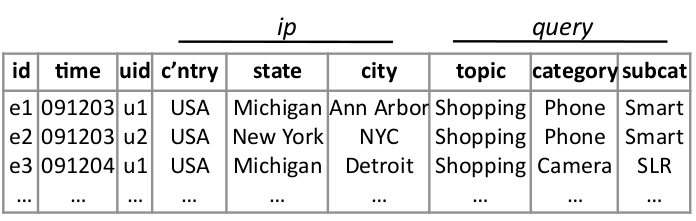
\includegraphics[width=3.5in]{picture/ch_datacube_mr/dataset_table} 
\caption{层次型数据集的表结构}\label{dataset_table1} 
\end{figure} 

因此这里针对层次型的数据数据集对生成 pipeline 的方法进行改进,该方法可解决pipeline之间长度差别过大的问题,并且同样简单有效。

%以下继续沿用图 \ref{dataset_table1} 作为数据集进行说明。该数据集的 lattice 如图\ref{dataset_lattice1} 所示。

%\begin{figure}[!htb]
%\centering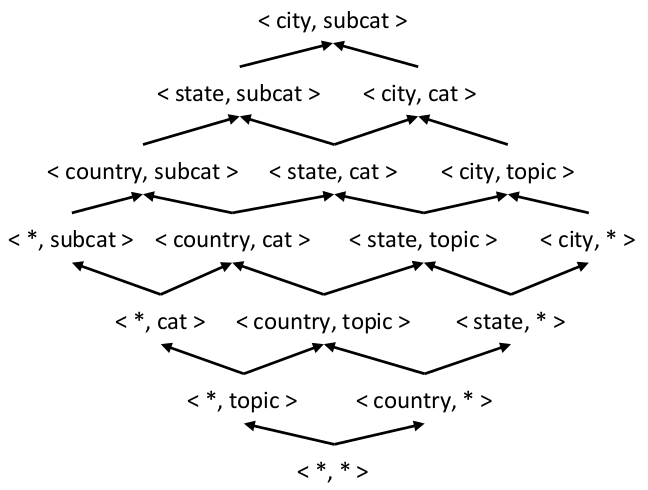
\includegraphics[width=3in]{picture/ch_datacube_mr/dataset_lattice} 
%\caption{层次型数据集的lattice}\label{dataset_lattice1} 
%\end{figure} 

在图\ref{dataset_table1}的数据集中,共有6个维属性,将这6个属性从0开始编号,如表\ref{attribute_no}所示。

\begin{table}[!htb]
\begin{center}
\begin{tabular}{|c|c|c|c|c|c|}
\hline 
Country & State & City & Topic & Category & Subcategory \\ 
\hline 
0 & 1 & 2 & 3 & 4 & 5 \\ 
\hline 
\end{tabular} 
\end{center}
\caption{数据集属性编号}\label{attribute_no}
\end{table}

对属性编号后,lattice 中的各个 region 可用编号组成的字符串表示。如 Region(state, category) 可用字符串 ``0 1 * 3 4 *" 表示。又如 Region(country, subcategory) 可用字符串 ``0 * * 3 4 5"表示。即对于要进行 GroupBy 的维属性在字符串中以编号出现,其他维属性则以 * 出现。由于数据集具有层次型,因此不可忽略该属性的前置属性。即 GroupBy(city) 时,默认等于 GroupBy(country, state, city),因此字符串中要出现 country 与 state。图 \ref{sorted_region}(a) 是将 lattcie 转化成字符串并按字典顺序排序后的结果。对字符串排序后的结果发现这样的顺序正好有 PipeSort 的特性。每4个字符串就刚好构成一个pipeline。图\ref{sorted_region}(b)中每个红色方框表示一个pipeline。

\begin{figure}[!h] 
\centering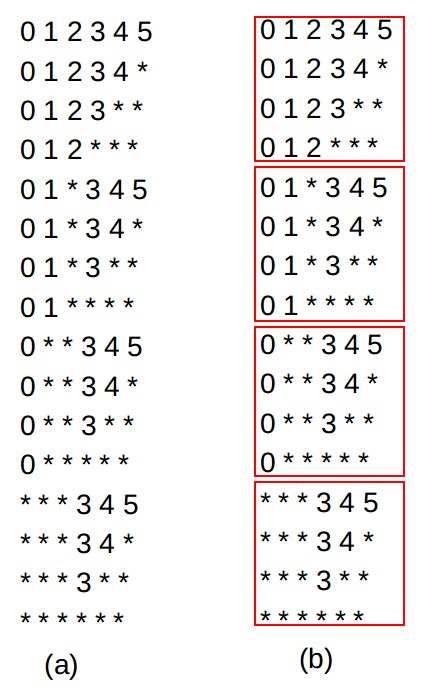
\includegraphics[width=1.9in]{picture/ch_terasort_mr/sorted_region} 
\caption{按字符串顺序排序的Region}\label{sorted_region} 
\end{figure}

这样的一种将region转化成字符串再排序的方法,对于层次型的数据集非常适用,因为它们具有层次型特征,在对字符串排序后,根据排序结果能直接形成 pipeline 。由于数据集的层次是既定的,因此形成的每个 pipeline 之间的 region 的数量基本是相等的,这样每个 reducer 要计算的 region 也是相对平均的。

因此这里建议,对于非层次型的数据集可使用 \cite{wang2013scalable} 中的方法形成 pipeline 方案,而对于层次型的数据集则使用region转换成字符串排序后形成的pipeline 方案。图\ref{greedy_pipeline} 和 图\ref{sort_pipeline} 分别为使用随机贪心和字符串排序生成的pipeline方案,图中使用红线划分了各个pipeline。从图中可看出,使用字符串排序生成的pipeline,各个pipeline的长度是相等的,更为均匀。


\begin{figure}[!htb]
\begin{tabular}{cc}

\begin{minipage}[t]{0.5\textwidth}
\centering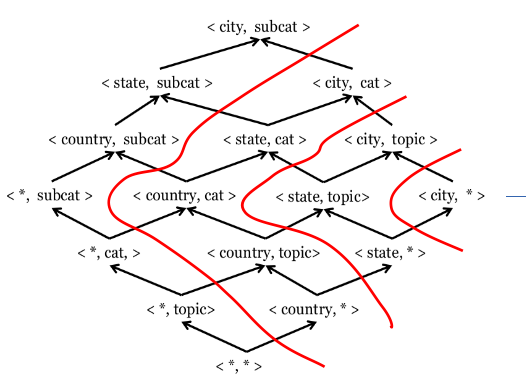
\includegraphics[width=3in]{picture/ch_terasort_mr/greedy_pipeline} 
\caption{随机贪心生成的pipeline}\label{greedy_pipeline} 
\end{minipage}

\begin{minipage}[t]{0.5\textwidth}
\centering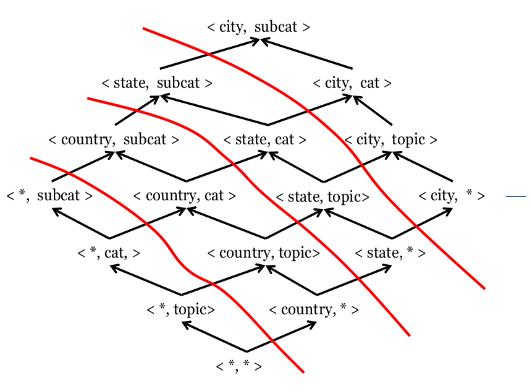
\includegraphics[width=3in]{picture/ch_terasort_mr/sort_pipeline} 
\caption{字符串排序生成的pipeline}\label{sort_pipeline} 
\end{minipage}

\end{tabular}
\end{figure}

pipeline方案形成后,即可与MapReduce结合进行数据立方的计算。由于MapReduce的分布式特性,它能并行处理多条pipeline,也就是每个reduce函数都处理与一条pipeline相关的数据。下面以 $ABCD\rightarrow ABC\rightarrow AB\rightarrow A$ 这个pipeline,e1=[a0, b0, c0, d0, m0]这条记录为例,分析使用PipeSort计算数据立方时 mapper 的输出,因为mapper的输出决定了各个reduce函数接收的数据。在e1 记录中,a0,b0,c0,d0分别对应属性A,B,C,D,它们是维属性,无层次型关系。m0对应的属性M为度量属性。以下暂不考虑数据的划分。

由于 PipeSort 的使用,mapper 的输出不再是映射所有的 region,而仅需要映射 每个pipeline 中的一个 region 即可。在这里 mapper 的key值选择 pipeline的末尾region 作为映射,而将剩余属性的值以及度量值放在value中。因此对于记录e1,mapper输出的key为[region\_id, a0],value的输出为[b0, c0, d0, m0]。根据MapReduce的机制,具有相同group值的数据都会放在同一个reduce函数中计算,因此Group(A=a0)的数据都放在同一个reduce函数中计算。由于value中包含了pipeline的其他属性BCD的值,以及度量属性M的值,并且用户可重载MapReduce的函数,令value按照一定要求进行排序,因此在Group(A=a0)的reduce函数中,可对数据进行一次扫描且只用少量内存,即可计算这条pipeline中与A=a0值相关的其他group。

倘若上述的pipeline映射的不是region(A),而是pipeline中其他的region,例如region(AB),即mapper输出的key值为属性AB组成的值,那么 region(A)的每一个group都被拆分到多个reduce函数中,导致之后还需要进行合并操作,并且这样也无法计算一条完整的pipeline,因为这条pipeline到了属性AB就被终止了。因此在pipesort与分布式数据立方结合的计算中,mapper 输出的 key值为pipeline 末尾region对应的属性值,value 值为起始region的属性除去 末尾region的属性后对应的属性值以及度量值。起始region 指pipeline中第一个region,末尾region指pipeline中最后一个region。在$ABCD\rightarrow ABC\rightarrow AB\rightarrow A$ 这个pipeline中,ABCD为起始region,A为末尾region。



\subsection{TeraSort与PipeSort的整合}

由于TSP-Cube使用了TeraSort,TeraSort会将大group进行划分,因此之后必定需要合并操作。所以 TSP-Cube 需要执行3次MapReduce完成数据立方的计算。第一轮 MapReduce 是采样以及选取分界点,第二轮 MapReduce 结合 PipeSort 计算数据立方,第三轮MapReduce 对上一轮输出的结果进行合并。

由于将 TeraSort 与 PipeSort 结合,因此这里第一轮 MapReduce 的采样数据与前面不考虑 PipeSort 的采样有所不同。在之前的章节中提到,使用TeraSort,第一轮与第二轮 mapper 输出的key值需要一致,才能进行比较,从而确定数据落到哪个reducer上。由于第二轮的 MapReduce 与 PipeSort 结合,不再需要映射所有的region,只需要映射pipeline末尾的region,因此第一轮采样的数据也不需要映射所有的region,只需要映射pipeline末尾的region即可。并且这两轮MapReduce中 mapper的输出依然是[region\_id, group\_value, tuple\_id or measure\_value] 这样的复合键。


%这里需要为 MapReduce 的机制进行一些说明。在默认的 MapReduce 中,只有具有相同 key 值的数据才会放在同一个 reduce 函数中计算。而在 TSP-Cube 第二轮 MapReduce 中 mapper 输出的 key 值为 [region\_id, group\_value, tuple\_id or measure\_id],是一个复合键。按照默认规定,必须这3个值都相同才能放在同一个 reduce 函数内计算。但其实 MapReduce 的框架为此提供了灵活的变化。用户可重载 GroupPartitioner 函数,此函数是定义在同一个 reducer 内,具有什么特征的数据会被放在同一个 reduce 函数中计算。由于TSP-Cube 的特殊性,这里需要重载 GroupPartioner,规定在同一个reducer内,只要 region\_id 和 group\_value 相同的数据即可放在同一个 reduce 函数内计算。

最后进行第三轮的 MapReduce,将被划分的数据进行合并。这里合并的方法非常简单,并且实验证明也是很高效的。合并的方法与 MapReduce 做单词统计是类似的,因为第二轮 MapReduce 输出的 key 是 region\_id 和 group\_value,输出的 value 是 measure\_value。因此在第三轮的 MapReduce 中,只要将第二轮输出的数据读入,对相同 region\_id 和 group\_value 的数据做一次合并即可,这个过程与单词统计是一样的。虽然上一轮将部分的 group 进行划分,但是这个划分的数量是有限,因此合并过程花费时间较少。


TSP-Cube 第一轮与第二轮的 MapReduce 的伪代码如算法\ref{tscube_mr1}、\ref{tscube_mr2} 所示。

%将TeraSort 与pipeline结合,若末尾的region过大,

%TSP-Cube 可对大的group 进行划分,pipesort 可减少中间数据的产生,并且将多个 group 放在同一个 reduce 函数中计算。由于 pipesort 的使用,无论是采样还是数据立方的计算,mapper 的输出不再是映射所有的 region,而仅需要映射这个pipeline 中的一个 region 即可。下面以 ABCD-\textgreater ABC-\textgreater AB-\textgreater A 这个pipeline,e1=[a0, b0, c0, d0, m0]这条记录为例,分别分析采样与数据立方计算时 mapper 的输出。以下将Tera Sort 与 PipeSort结合计算数据立方的方法称为 TSP-Cube。

%在TSP-Cube 的第一轮 MapReduce中,mapper 输出的样本的 key值应为[region\_id, group\_value, tuple\_id or measure\_value]。这里对应上述的pipeline 和记录,mapper 输出的key应为 [Region(A)\_id, a0, tuple\_id or measure\_value]。

%在TSP-Cube 的第二轮 MapReduce 中,mapper 输出的key应与第一轮是一致的,因此mapper 输出的key为[Region(A)\_id, a0, tuple\_id or measure\_value],输出的value则为[b0, c0, d0] 这样的组合键。在上面的章节中提到,MapReduce的机制较为灵活,可重载 GroupComparator 函数,令只要有相同 region\_id 和 group\_value 的数据都放在同一个 reduce 函数中。因此在同一个 reducer 中,对于属性 A 具有相同值的数据都会放在同一个 reduce 函数里,即使它们的 tuple\_id 或 measure\_value 不同。

%由于 pipesort 的使用,mapper 的输出不再是映射所有的 region,而仅需要映射 pipeline 中的一个 region 即可,而在这里 mapper 的key值选择了 region(A) 作为映射,而将剩余属性的值放在了value中。若在单机上使用 pipeline 计算数据立方,只要将数据按照 ABCD 这样的属性顺序排序,然后对数据扫描一遍即可计算 GroupBy(ABCD),GroupBy(ABC),GroupBy(AB),GroupBy(A)的值。但是在分布式中,需要对数据进行划分,而我们希望数据的划分能在满足 pipeline 计算的同时每个分块尽可能地小。这样可减轻 reducer 在shuffle 和 sort 阶段的负担,提高计算效率。为了满足 ABCD-\textgreater ABC-\textgreater AB-\textgreater A 这个 pipeline 的计算,具有相同属性 A 的值的数据必定要放在同一个分块内(除非由于这个 group 过大,被分界点划分了)。那么数据则根据属性A的值被分成若干个分块,每个分块上都可进行 pipeline 的计算,并且互相是不影响的,从而实现了多个pipeline的并行计算。

%对于任何一条 pipeline,起始的region 一定是属性数量最多的,末尾的reigon一定是属性数量最少的。对于每条记录,都要与每个pipeline做映射。在数据立方的计算中,mapper 输出的 key值为 末尾region对应的属性值与tuple\_id 或 measure\_id的组合,mapper 输出的value 值为起始region中的属性除去 末尾region的属性后对应的属性值。如图\ref{dataset_table} 对应的数据集,生成的pipesort方案如图\ref{sorted_region}所示共有4个pipeline,因此每条记录都要映射4个键值对。

%\section{TSP-Cube 实现伪代码}



{\renewcommand\baselinestretch{1} 

\begin{algorithm}[htbp]
\caption{TSP-Cube Estimate Algorithm}
\label{tscube_mr1}
{\fontfamily{\familydefault}\selectfont

	\begin{algorithmic}[1] %每行显示行号
    \Function {ESTIMATE-MAP}{e}
    	\State e is a tuple in the dataset
    	\ForAll {Pipeline in PipeSort-Solution}
    		\State FR=first region of the pipeline
    		\State LR=last region of the pipeline
        	\State k=[LR\_RegionID(e),LR\_GroupValue(e),TupleID(e) or MeasureValue(e)]
        	\State EMIT([k],[arbitrary value])
        \EndFor
   	 \EndFunction
   	 \State
     \Function {ESTIMATE-REDUCE}{k1,k2,k3...}
     	\While {t < SampleSize}
     		\If {${k}_{t}$ is the $i\times \left \lceil \frac{SampleSize}{BoundaryNum} \right \rceil th$ object }
     		 \State	
     		 EMIT([${k}_{t}$],[arbitrary value]); i++
     		\EndIf
     		\State t++
     	\EndWhile
     \EndFunction
	\end{algorithmic}	
}
\end{algorithm}

\par}


%\textcolor{white}{--------------------------------------
\phantom{--------------------------------------
----------------------------------------------------------------------------------------------------------------
----------------------------------------------------------------------------------------------------------------
----------------------------------------------------------------------------------------------------------------
----------------------------------------------------------------------------------------------------------------
----------------------------------------------------------------------------------------------------------------
----------------------------------------------------------------------------------------------------------------
----------------------------------------------------------------------------------------------------------------
----------------------------------------------------------------------------------------------------------------
----------------------------------------------------------------------------------------------------------------
----------------------------------------------------------------------------------------------------------------
----------------------------------------------------------------------------------------------------------------
---------------------------------------------------------------------------------------------------------
}


{\renewcommand\baselinestretch{1} 

\begin{algorithm}[H]
\caption{TSP-Cube Materialize Algorithm}
\label{tscube_mr2}
{\fontfamily{\familydefault}\selectfont

	\begin{algorithmic}[1] %每行显示行号
    \Function {Materialize-MAP}{e}
    	\State e is a tuple in the dataset
    	\ForAll {Pipeline in PipeSort-Solution}
    		\State FR=first region of the pipeline
    		\State LR=last region of the pipeline
        	\State k=[LR\_RegionID(e),LR\_GroupValue(e),TupleID(e) or MeasureValue(e)]
        	\State v=[FR\_GroupValue(e)]
        	\State EMIT([k],[v])
        \EndFor
   	 \EndFunction
   	 \State
     \Function {Materialize-REDUCE}{k,[v1,v2,v3...]}
     	%\State Pipeline Calculate 
     	\ForAll {${v}_{i}$}
     		\If {${v}_{i} \neq {v}_{i-1}$}
     			\State
     			CALCULATE corresponding group and EMIT result
     		\EndIf
     	\EndFor
     \EndFunction
	\end{algorithmic}	
}
\end{algorithm}

\par}









